\section{Introduction}
\label{sec:intro}

\begin{comment}
-- OUTLINE
a. Define counterfactual. counterfactuals are how we understand stuff (cite psychology papers) and run decent experiments. Counterfactuals are hard in the real world (cite pearl), but easy if we're analyzing a model
b. Current counterfactuals in NLP: useful for training and eval (contrast sets), but done by hand. Too much work, relies on creativity, may miss stuff. For explanations: adversarial examples, or simple word substitutions.
c. We formalize the task of counterfactual generation: given x, produce \xp, and then rank according to the task. We train a model to do this (some detail).
d. we apply the model to training, eval, explanations. summary of results. Important: compare to counterfactuals created by hand, this is better and faster
\end{comment}

\begin{figure}[t]
\centering
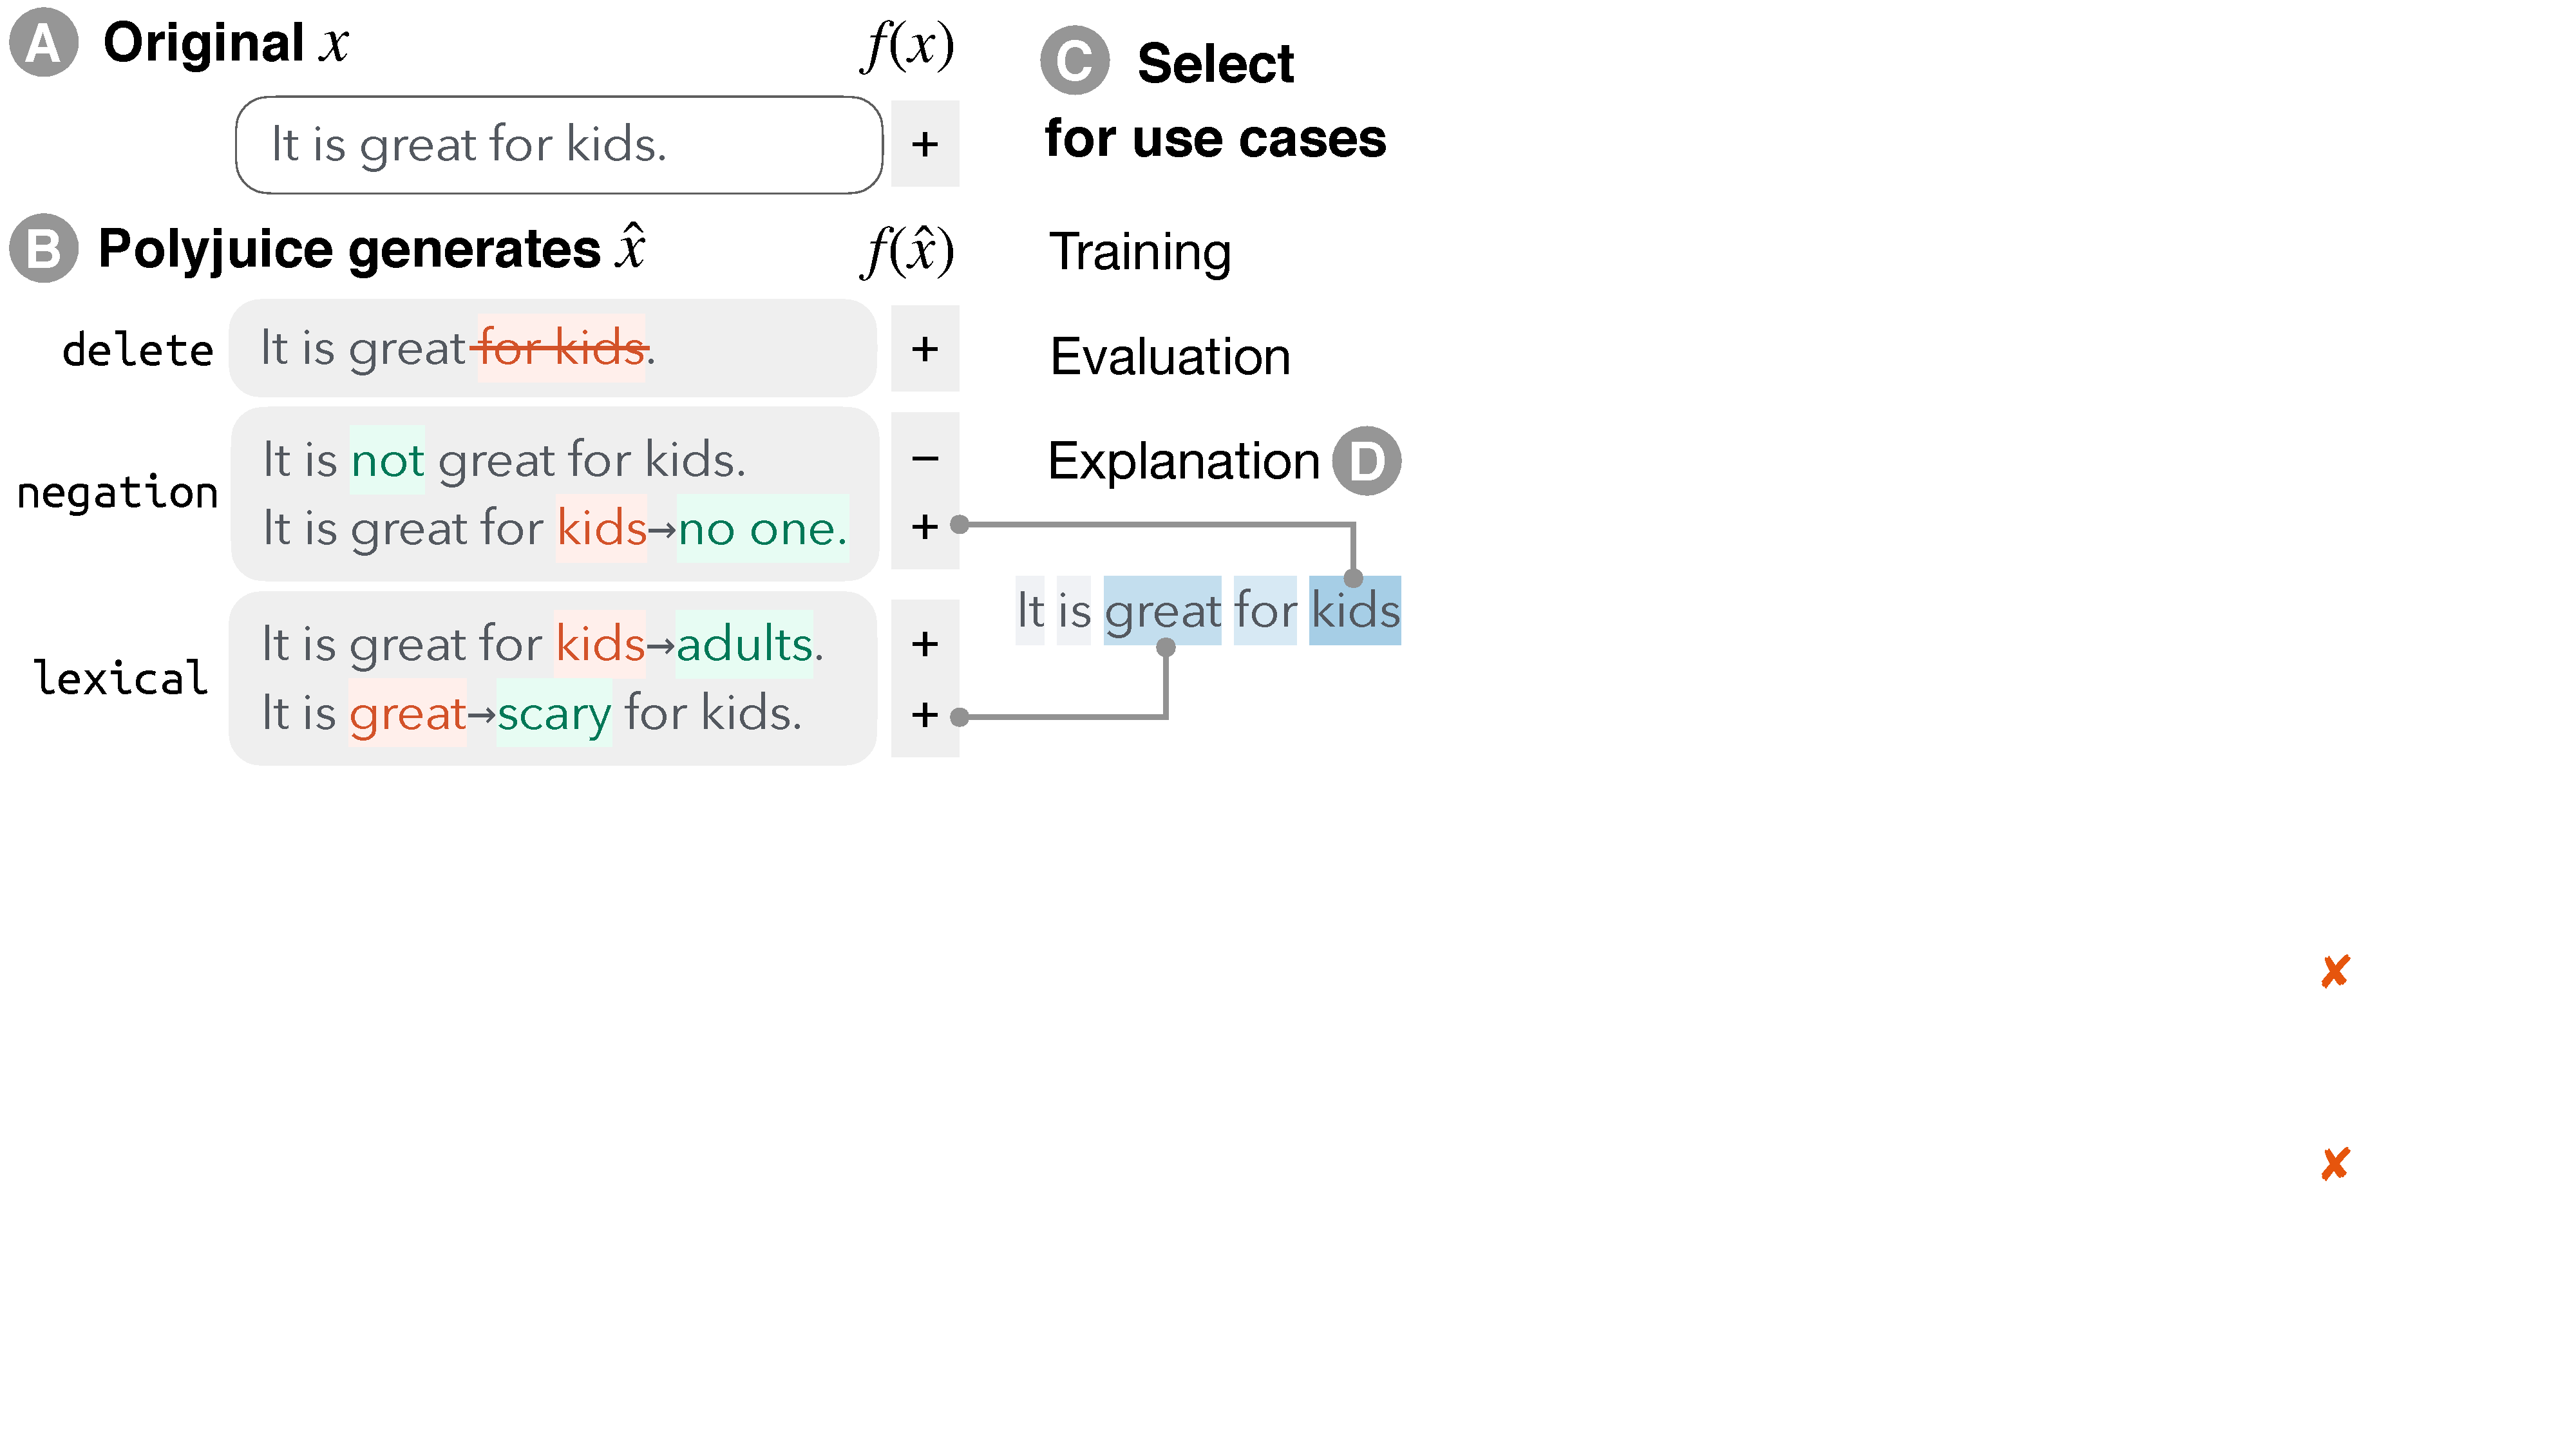
\includegraphics[trim={0 18cm 30.5cm 0cm},clip, width=1\columnwidth]{figures/teaser}
\vspace{-15pt}
\caption{
The process of \sysname on a sentiment analysis instance.
Given an original $x$ (A), we generate (B) a large number of $\xp$-s, which are then (C) sorted and selected in different ways for downstream use cases.
For example, as counterfactual explanations (D), we can select $\xp$ that complement the feature weights:  though both ``great'' and ``kids'' are deemed important, the selected $\xp$ show that changing them do not always result in model prediction change and reveal model errors.
}
\vspace{-15pt}
\label{fig:teaser}
\end{figure} 
 

Counterfactual reasoning --- mentally simulating what \emph{would have happened} if conditions were different --- is a common tool for making causality assessments~\cite{kahneman}, which in turn are crucial for explanation~\cite{miller}, evaluation, and model training. For example, in Figure~\ref{fig:teaser}, $x=$ \exinline{It is great for kids.} is perturbed into $[\xp_1, \xp_2, ...]$ in such a way that the changes from $x$ to $\xp_i$ brings various insights by simulating what would have happened if $x$ was different.

Applications of counterfactual reasoning to Natural Language Processing (NLP) generally specify the relationship $x \rightarrow \xp$, and then ask humans to manually create counterfactuals $\xp$, or perturbation functions that generate $\xp$.
For example, \citet{gardner2020contrast} and \citet{kaushik2019learning} ask humans to create counterfactuals $\xp$ that are as close to $x$ as possible \emph{but have a different groundtruth label}, to improve training and evaluation. 
Similarly, \citet{wu2019errudite} and \citet{checklist:acl20} ask humans to create counterfactual-generating functions such as ``remove negation'' or ``add irrelevant information'' in order to verify or test specific model behaviors (\eg whether models handle negation appropriately).
These are costly to generate, and may miss important patterns due to their reliance on human creativity (\eg humans may cover \swap{great}{not great}, but can easily miss \swap{kids}{no one} in Figure~\ref{fig:teaser}B).
Though it is cheaper to automate the process with parsing templates~\cite{li2020linguistically}, the templates usually have limited coverage on either the patterns-to-perturb, or the applicable data points.
Adversarial examples are a different form of counterfactual reasoning: $x$ and $\xp$ have different model predictions \emph{despite} being semantically equivalent --- i.e. most perturbations are word replacements or other forms of paraphrasing~\cite{iyyer2018adversarial, ribeiro2018semantically}.
%In this rare case where counterfactuals can reliably be produced automatically, humans are not able to create counterfactuals with the desired property as well as automatic methods~\cite{ribeiro2018semantically}, even though they excel at evaluating such counterfactuals.
%TODO: NEed to say something about Li et al 2020 Linguistically-Informed Transformations (LIT): A Method for Automatically Generating Contrast Sets, maybe something about word substitution



In this work, we formalize the task of \emph{automatic counterfactual generation}, where given an input $x$, the goal is to produce a set of counterfactuals $\xp$-s with reasonable relationships $x \rightarrow \xp_i$. 
We frame the task as text generation, and finetune GPT-2~\cite{radford2019language} on a dataset of  $(x, \xp)$ pairs, such that it learns to generate general purpose $\xp$-s that are \emph{realistic}, \emph{diverse}, and \emph{close to $x$}.
We also allow for targeted counterfactuals, by specifying where the perturbation occurs in the sentence~\cite{donahue2020enabling} and using \tagstrs such as \ctrltag{negation} or \ctrltag{delete} (Figure~\ref{fig:teaser}B). 
The produced counterfactuals are then ranked and selected according to the applications of interest (Figure~\ref{fig:teaser}C).

We demonstrate the usefulness of \sysname in facilitating counterfactual training and evaluation. 
By asking humans to \emph{label} diverse counterfactuals rather than create them from scratch \cite{gardner2020contrast, kaushik2019learning}, we produce high-quality contrast sets~\cite{gardner2020contrast} at a fraction of the cost, as well as training data that improves generalization in three different tasks (Sentiment Analysis \sst, Natural Language Inference \nli, and Duplicate Question Detection \qqp), when compared to adding the same amount of non-counterfactual data.

% (on Sentiment Analysis \sst, Natural Language Inference \nli, and Duplicate Question Detection \qqp), we observe that asking humans to validate \emph{diverse} counterfactuals is enough to produce high-quality contrast sets~\cite{gardner2020contrast} and training data that improves generalization accuracy (measured by out-of-domain datasets, challenge sets, contrast sets, and CheckLists~\cite{checklist:acl20}).

% We \emph{propose appropriate selection strategies}, and demonstrate \sysname in three scenarios that require counterfactual reasoning: \emph{training, evaluation, and explanation}.
% For training and evaluation (on Sentiment Analysis \sst, Natural Language Inference \nli, and Duplicate Question Detection \qqp), we observe that asking humans to validate \emph{diverse} counterfactuals is enough to produce high-quality contrast sets~\cite{gardner2020contrast}, and training data that improves generalization accuracy (measured by out-of-domain datasets, challenge sets, contrast sets, and CheckLists~\cite{checklist:acl20}).
% Compared to the more difficult task of \emph{creating} counterfactuals, the validation is \emph{at least} 40\% more effective in terms of creation time.
%, even after aggressive filtering.
% (30 seconds for validating three $\xp$ around one $x$) 

We also demonstrate how \sysname can produce high quality \emph{black-box counterfactual explanations}.
Such explanations have been elusive in NLP, despite evidence from social science research \cite{miller} indicating that they may be more intuitive than feature attribution or attention maps, or at least be complementary to these methods. 
% We prioritize counterfactuals with \emph{abnormal} model behaviors, \ie the actual changes in prediction do not match the expectation.
%(measured by sentence similarity or perturbed feature weights.)
We validate this hypothesis in user study, and observed that expert users only did slightly better than random (accuracy: $55 \pm 6\%$) at predicting what a model would do on \sysname counterfactuals, even after seeing SHAP explanations \cite{NIPS2017_7062} and manually exploring the model's behavior. 
This indicates that seeing such explanations would add a lot of information that users are currently missing (much of which consisting of mistaken model predictions) when they perform manual counterfactual analysis and use feature attribution methods.


% we observe that \sysname explanations can complement popular feature attribution methods and highlight their blind spots.
% After viewing SHAP weights~\cite{NIPS2017_7062} and interacting with the model, experts still could not predict model behaviors on counterfactuals selected for explanations, and missed 5\% and 25\% more cases than the human-generated or random baselines.
